\documentclass[11pt]{article}


\usepackage{soul}
\usepackage[T1]{fontenc}
\usepackage{amsfonts, amsmath, amssymb}
\usepackage{multirow}
\usepackage{epsfig}
\usepackage{subfigure}
\usepackage{subfloat}
\usepackage{graphicx}

\usepackage{booktabs}
\usepackage{longtable}

\usepackage{verbatim, rotating, paralist}
\usepackage{enumerate}

\usepackage{natbib}


\usepackage{pdfsync}
\usepackage{latexsym}
\usepackage{amsthm}
\usepackage{mathabx}
   
\usepackage{stmaryrd}
\usepackage{mathrsfs}
\usepackage{dsfont}


\usepackage{parskip}
\usepackage{anysize, indentfirst, setspace}
\usepackage[right=2cm, left=2cm, top=3.25cm, bottom=3.25cm]{geometry} 
\usepackage{epigraph}
\usepackage{appendix}


\renewcommand{\topfraction}{.85}
\renewcommand{\bottomfraction}{.7}
\renewcommand{\textfraction}{.15}
\renewcommand{\floatpagefraction}{.66}
\renewcommand{\dbltopfraction}{.66}
\renewcommand{\dblfloatpagefraction}{.66}







\begin{document} 


\singlespacing
\setlength{\parindent}{0in}
\setlength{\parskip}{0in}




%--------------------------------------------HEADER-----------------------------------------------------------------------%
\begin{center}
	\large{\so{LATIN AMERICAN HISTORY} }\\
	\large{\so{Week 1: Pre-Colonial America} }\\
\end{center}



\vspace{.3in}
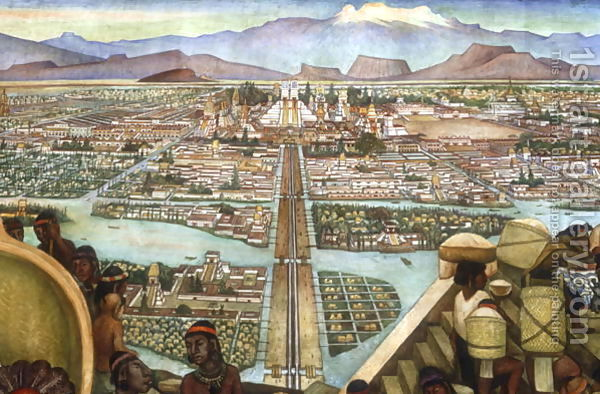
\includegraphics[width=3in, clip=true,trim= 0in 0in .5in 0in]{Aztec2.jpg}
\hspace*{.5in}
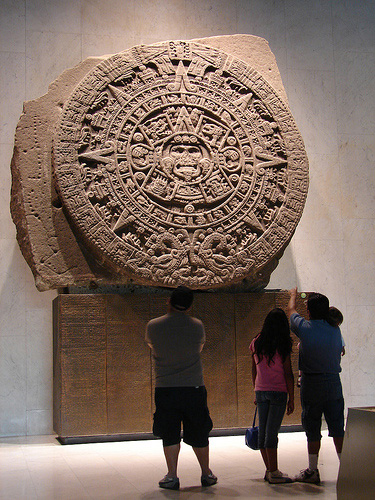
\includegraphics[width=2.5in]{Aztec1.jpg}\\
\footnotesize  Painting \emph{The Great Tenochtitlan}, by Diego Rivera (1945)  \hspace*{.4in}   Aztec Calendar Stone, Museo Nacional de Antropologia,\\
\hspace*{3.55in} Mexico City


\vspace{.3in}
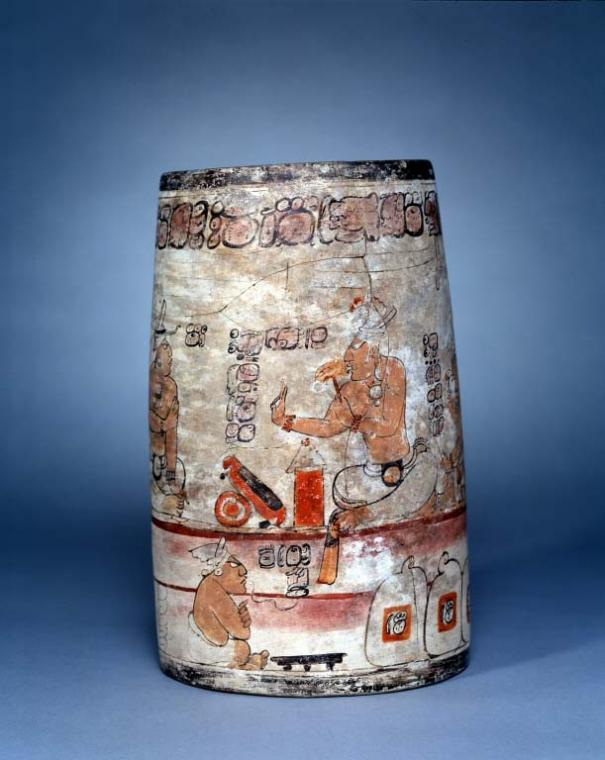
\includegraphics[width=3in,clip=true,trim= .3in .2in .3in 0.9in]{Maya2.jpg} 
\hspace*{.4in}
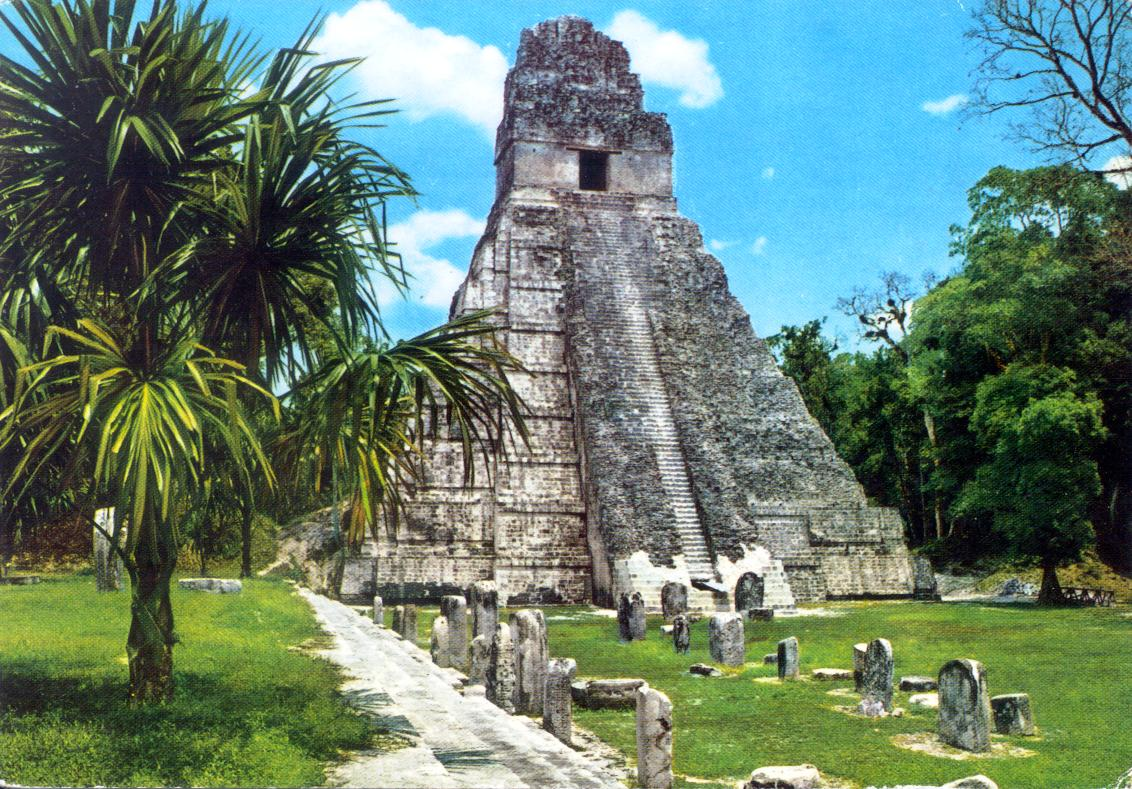
\includegraphics[width=3.2in]{Tikal.jpg} \\
Vase with Palace Scene, AD 600-800, Denver Art Museum \hspace*{.18in}  Photograph of Tikal, Mexico


\vspace{.3in}
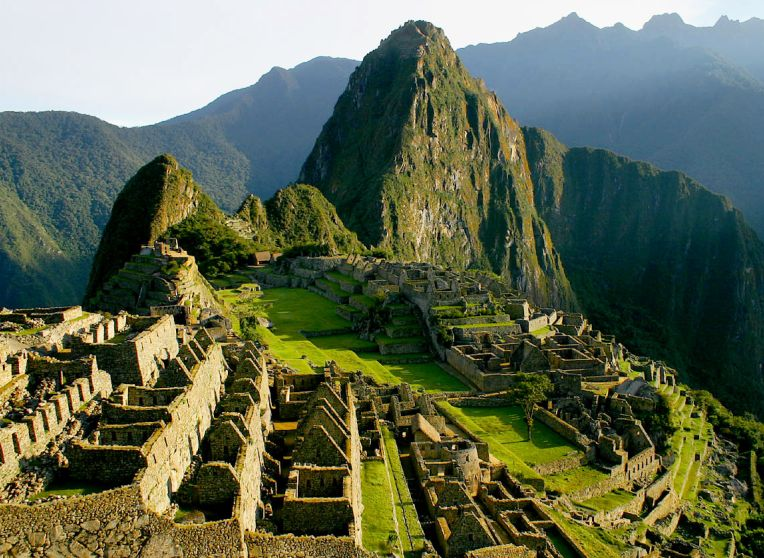
\includegraphics[width=2.5in]{MP1.jpg}
\hspace*{.2in}
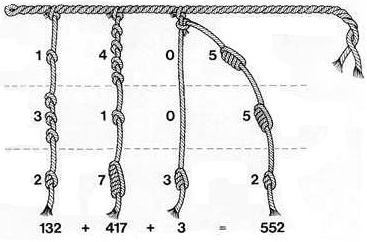
\includegraphics[width=2in]{Inca1.png}
\hspace*{.2in}
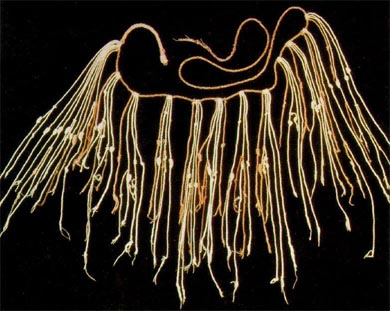
\includegraphics[width=2in]{Inca2.jpg}\\
Photograph of Macchu Picchu, Peru  \hspace*{.6in} Diagram of Inca counting knots   \hspace*{.5in} Photograph of Inca knots




\end{document}















